\begin{task}
Wyznacz współczynniki trygonometrzycznego szeregu fouriera dla okresowego sygnału $f(t)$ przedstawionego na rysunku

\begin{figure}[H]
\centering
\begin{tikzpicture}
  %\draw (0,0) circle (1in);
  \draw[->] (-3.0,+0.0) -- (+5.0,+0.0) node[right] {$t$};
  \draw[->] (+0.0,-1.5) -- (+0.0,+2.0) node[above] {$f(t)$};
  \draw[scale=1.0,domain=-1.5:-1.0,samples=100,smooth,variable=\x,red,thick] plot ({\x},{0.0+1*sin(\x*180.0/3.141592*1*3.141592/1.0)});
  \draw[-,red, thick] (-1.0,0.0) -- (0.0,0.0);
  \draw[scale=1.0,domain=0.0:1.0,samples=100,smooth,variable=\x,red,thick] plot ({\x},{0.0+1*sin(\x*180.0/3.141592*1*3.141592/1.0)});
  \draw[-,red, thick] (1.0,0.0) -- (2.0,0.0);
  \draw[scale=1.0,domain=2.0:3.0,samples=100,smooth,variable=\x,red,thick] plot ({\x},{0.0+1*sin(\x*180.0/3.141592*1*3.141592/1.0)});
  \draw[-,red, thick] (3.0,0.0) -- (3.5,0.0);
  \draw[-,red, dashed] (-2.0,1.0) -- (4.0,1.0);
  %\draw[-] (-1.0-0.1,-0.1)--(-1.0+0.1,0.1) node[midway, below, outer sep=10pt,align=center] {$-\frac{T}{2}$};
  \draw[-] (-1.0-0.1,-0.1)--(-1.0+0.1,0.1) node[midway, below, outer sep=5pt] {$-\frac{T}{2}$};
  \draw[-] (+1.0-0.1,-0.1)--(+1.0+0.1,0.1) node[midway, below, outer sep=5pt] {$\frac{T}{2}$};
  \draw[-] (+2.0-0.1,-0.1)--(+2.0+0.1,0.1) node[midway, below, outer sep=5pt] {$T$};
  \draw[-] (-0.1,+1.0-0.1)--(+0.1,+1.0+0.1) node[midway, left] {$A$};

\end{tikzpicture}
\end{figure}

W pierwszej kolejności należy opisać sygnał za pomocą wzoru:

\begin{equation}
f(x)=\begin{cases}A \cdot sin\left( \frac{2\pi}{T} \cdot t\right) & t \in \left ( 0+k \cdot T; \frac{T}{2}+k \cdot T \right ) \\
0 & t \in \left ( \frac{T}{2}+k \cdot T; T+k \cdot T \right )\end{cases} \wedge k \in C %\mathbb{C}
\end{equation}

Współczynnik $a_0$ wyznaczamy ze wzoru

\begin{equation}
a_0=\frac{1}{T}\int_{T}f(t) \cdot dt
\end{equation}

Podstawiamy do wzoru wzór naszej funkcji w pierwszym okresie $k=0$

%\begin{equation}
%\begin{aligned}
\begin{align*}
a_0&=\frac{1}{T}\int_{T}f(t) \cdot dt\\
&=\frac{1}{T}\left(\int_{0}^{\frac{T}{2}}A \cdot sin\left( \frac{2\pi}{T} \cdot t\right) \cdot dt 
+ \frac{1}{T}\int_{\frac{T}{2}}^{T}0 \cdot dt \right)\\
&=\frac{A}{T}\left(\int_{0}^{\frac{T}{2}}sin\left( \frac{2\pi}{T} \cdot t\right) \cdot dt 
+ 0 \right)\\
&=\frac{A}{T}\int_{0}^{\frac{T}{2}}sin\left( \frac{2\pi}{T} \cdot t\right) \cdot dt\\
&=\begin{Bmatrix*}[l]
z&=\frac{2\pi}{T} \cdot t\\
dz&=\frac{2\pi}{T} \cdot dt\\
dt&=\frac{dz}{\frac{2\pi}{T}}
\end{Bmatrix*}\\
&=\frac{A}{T}\int_{0}^{\frac{T}{2}}sin\left( z\right) \cdot \frac{dz}{\frac{2\pi}{T}}\\
&=\frac{A}{T\cdot \frac{2\pi}{T}}\int_{0}^{\frac{T}{2}}sin\left( z\right) \cdot dz\\
&=\frac{A}{2\pi}\cdot \left(\left . -cos\left( z\right) \right|_{0}^{\frac{T}{2}}\right)\\
&=-\frac{A}{2\pi}\cdot \left(\left . cos\left( \frac{2\pi}{T} \cdot t\right) \right|_{0}^{\frac{T}{2}}\right)\\
&=-\frac{A}{2\pi}\cdot \left( cos\left( \frac{2\pi}{T} \cdot \frac{T}{2}\right) - cos\left( \frac{2\pi}{T} \cdot 0\right)\right)\\
&=-\frac{A}{2\pi}\cdot \left( cos\left( \pi\right) - cos\left( 0\right)\right)\\
&=-\frac{A}{2\pi}\cdot \left( -1 - 1\right)\\
&=-\frac{A}{2\pi}\cdot \left( -2\right)\\
&=\frac{A}{\pi}\\
\end{align*}
%\end{aligned}
%\end{equation}

Wartość współczynnika $a_0$ wynosi $\frac{A}{\pi}$

Współczynnik $a_k$ wyznaczamy ze wzoru

\begin{equation}
a_k=\frac{2}{T}\int_{T}f(t) \cdot cos\left( k \cdot \frac{2\pi}{T} \cdot t\right) \cdot dt
\end{equation}

Podstawiamy do wzoru wzór naszej funkcji w pierwszym okresie $k=0$

%\begin{equation}
%\begin{aligned}
\begin{align*}
a_k&=\frac{2}{T}\int_{T}f(t) \cdot cos\left( k \cdot \frac{2\pi}{T} \cdot t\right) \cdot dt\\
&=\frac{2}{T}\cdot\left(\int_{0}^{\frac{T}{2}}A \cdot sin\left( \frac{2\pi}{T} \cdot t\right) \cdot cos\left( k \cdot \frac{2\pi}{T} \cdot t\right) \cdot dt+\int_{\frac{T}{2}}^{T} 0 \cdot cos\left( k \cdot \frac{2\pi}{T} \cdot t\right) \cdot dt\right)\\
&=\frac{2}{T}\cdot\left(A \cdot \int_{0}^{\frac{T}{2}}sin\left( \frac{2\pi}{T} \cdot t\right) \cdot cos\left( k \cdot \frac{2\pi}{T} \cdot t\right) \cdot dt+\int_{\frac{T}{2}}^{T} 0 \cdot dt\right)\\
&=\begin{Bmatrix*}[l]
cos\left(x\right)&=\frac{e^{\jmath \cdot x}+e^{-\jmath \cdot x}}{2}\\
sin\left(x\right)&=\frac{e^{\jmath \cdot x}-e^{-\jmath \cdot x}}{2 \jmath }
\end{Bmatrix*}\\
&=\frac{2}{T}\cdot\left(A \cdot \int_{0}^{\frac{T}{2}} \frac{e^{\jmath \cdot \frac{2\pi}{T} \cdot t}-e^{-\jmath \cdot \frac{2\pi}{T} \cdot t}}{2\jmath} \cdot \frac{e^{\jmath \cdot k \cdot \frac{2\pi}{T} \cdot t}+e^{-\jmath \cdot k \cdot \frac{2\pi}{T} \cdot t}}{2} \cdot dt+0\right)\\
&=\frac{2}{T}\cdot\left(\frac{A}{2\cdot 2\jmath} \cdot \int_{0}^{\frac{T}{2}} \left(e^{\jmath \cdot \frac{2\pi}{T} \cdot t}-e^{-\jmath \cdot \frac{2\pi}{T} \cdot t}\right)\cdot \left(e^{\jmath \cdot k \cdot \frac{2\pi}{T} \cdot t}+e^{-\jmath \cdot k \cdot \frac{2\pi}{T} \cdot t}\right) \cdot dt\right)\\
&=\frac{2}{T} \cdot \frac{A}{2\cdot 2\jmath} \cdot \int_{0}^{\frac{T}{2}}
\left(e^{\jmath \cdot \frac{2\pi}{T} \cdot t} \cdot e^{\jmath \cdot k \cdot \frac{2\pi}{T} \cdot t} + e^{\jmath \cdot \frac{2\pi}{T} \cdot t} \cdot e^{-\jmath \cdot k \cdot \frac{2\pi}{T} \cdot t} - e^{-\jmath \cdot \frac{2\pi}{T} \cdot t} \cdot e^{\jmath \cdot k \cdot \frac{2\pi}{T} \cdot t} - e^{-\jmath \cdot \frac{2\pi}{T} \cdot t} \cdot e^{-\jmath \cdot k \cdot \frac{2\pi}{T} \cdot t} \right) \cdot dt\\
&=\frac{A}{T\cdot 2\jmath} \cdot \int_{0}^{\frac{T}{2}}
\left(e^{\jmath \cdot \frac{2\pi}{T} \cdot t + \jmath \cdot k \cdot \frac{2\pi}{T} \cdot t} + e^{\jmath \cdot \frac{2\pi}{T} \cdot t -\jmath \cdot k \cdot \frac{2\pi}{T} \cdot t} - e^{-\jmath \cdot \frac{2\pi}{T} \cdot t+ \jmath \cdot k \cdot \frac{2\pi}{T} \cdot t} - e^{-\jmath \cdot \frac{2\pi}{T} \cdot t -\jmath \cdot k \cdot \frac{2\pi}{T} \cdot t} \right) \cdot dt\\
&=\frac{A}{T\cdot 2\jmath} \cdot \int_{0}^{\frac{T}{2}}
\left(e^{\jmath \cdot \frac{2\pi}{T} \cdot t \cdot \left(1+k\right)} + e^{\jmath \cdot \frac{2\pi}{T} \cdot t \cdot \left(1 - k\right)} - e^{-\jmath \cdot \frac{2\pi}{T} \cdot t \cdot \left(1 -k\right)} - e^{-\jmath \cdot \frac{2\pi}{T} \cdot t \cdot \left(1+k\right)} \right) \cdot dt\\
&=\frac{A}{T\cdot 2\jmath} \cdot \int_{0}^{\frac{T}{2}}
\left(e^{\jmath \cdot \frac{2\pi}{T} \cdot t \cdot \left(1+k\right)} - e^{-\jmath \cdot \frac{2\pi}{T} \cdot t \cdot \left(1+k\right)} + e^{\jmath \cdot \frac{2\pi}{T} \cdot t \cdot \left(1 - k\right)} - e^{-\jmath \cdot \frac{2\pi}{T} \cdot t \cdot \left(1 -k\right)} \right) \cdot dt\\
&=\frac{A}{T} \cdot \int_{0}^{\frac{T}{2}}
\left( \frac{e^{\jmath \cdot \frac{2\pi}{T} \cdot t \cdot \left(1+k\right)} - e^{-\jmath \cdot \frac{2\pi}{T} \cdot t \cdot \left(1+k\right)}}{2\jmath} + \frac{e^{\jmath \cdot \frac{2\pi}{T} \cdot t \cdot \left(1 - k\right)} - e^{-\jmath \cdot \frac{2\pi}{T} \cdot t \cdot \left(1 -k\right)}}{2\jmath} \right) \cdot dt\\
&=\frac{A}{T} \cdot \int_{0}^{\frac{T}{2}}
\left( sin\left( \frac{2\pi}{T} \cdot t \cdot \left(1+k\right) \right) + sin\left( \frac{2\pi}{T} \cdot t \cdot \left(1 - k\right)\right) \right) \cdot dt\\
&=\frac{A}{T} \cdot \left( \int_{0}^{\frac{T}{2}}
 sin\left( \frac{2\pi}{T} \cdot t \cdot \left(1+k\right) \right) \cdot dt + \int_{0}^{\frac{T}{2}} sin\left( \frac{2\pi}{T} \cdot t \cdot \left(1 - k\right)\right) \cdot dt \right)\\
&=\begin{Bmatrix*}[l]
z_1&=\frac{2\pi}{T} \cdot t \cdot \left(1+k\right) & z_2&=\frac{2\pi}{T} \cdot t \cdot \left(1-k\right)\\
dz_1&=\frac{2\pi}{T} \cdot \left(1+k\right) \cdot dt & z_2&=\frac{2\pi}{T} \cdot \left(1-k\right) \cdot dt\\
dt&=\frac{dz_1}{\frac{2\pi}{T} \cdot \left(1+k\right)} \wedge k \neq -1& dt&=\frac{dz_2}{\frac{2\pi}{T} \cdot \left(1-k\right)} \wedge k \neq 1
\end{Bmatrix*}\\
&=\frac{A}{T} \cdot \left(\int_{0}^{\frac{T}{2}} sin\left( z_1 \right)\cdot \frac{dz_1}{\frac{2\pi}{T} \cdot \left(1+k\right)}  + \int_{0}^{\frac{T}{2}} sin\left( z_2\right) \cdot \frac{dz_2}{\frac{2\pi}{T} \cdot \left(1-k\right)}\right)\\
&=\frac{A}{T} \cdot \left(\frac{1}{\frac{2\pi}{T}\cdot \left(1+k\right)} \cdot \int_{0}^{\frac{T}{2}} sin\left( z_1 \right)\cdot dz_1 + \frac{1}{\frac{2\pi}{T} \cdot \left(1-k\right)} \cdot \int_{0}^{\frac{T}{2}} sin\left( z_2\right) \cdot dz_2 \right)\\
&=\frac{A}{T} \cdot \left(\frac{1}{\frac{2\pi}{T}\cdot \left(1+k\right)} \cdot \left( \left. -cos\left( z_1 \right) \right|_{0}^{\frac{T}{2}} \right) + \frac{1}{\frac{2\pi}{T} \cdot \left(1-k\right)} \cdot \left(\left. -cos\left( z_2\right) \right|_{0}^{\frac{T}{2}} \right) \right)\\
&=\frac{A}{T} \cdot \left(\frac{-1}{\frac{2\pi}{T}\cdot \left(1+k\right)} \cdot \left( \left. cos\left( \frac{2\pi}{T} \cdot t \cdot \left(1+k\right) \right) \right|_{0}^{\frac{T}{2}} \right) + \frac{-1}{\frac{2\pi}{T} \cdot \left(1-k\right)} \cdot \left(\left. cos\left( \frac{2\pi}{T} \cdot t \cdot \left(1-k\right)\right) \right|_{0}^{\frac{T}{2}} \right) \right)\\
&=\frac{A}{T} \cdot \left(\frac{-1}{\frac{2\pi}{T}\cdot \left(1+k\right)} \cdot \left( cos\left( \frac{2\pi}{T} \cdot \frac{T}{2} \cdot \left(1+k\right) \right) - cos\left( \frac{2\pi}{T} \cdot 0 \cdot \left(1+k\right) \right) \right) \right.\\
&\left.+ \frac{-1}{\frac{2\pi}{T} \cdot \left(1-k\right)} \cdot \left( cos\left( \frac{2\pi}{T} \cdot \frac{T}{2} \cdot \left(1-k\right)\right) -  cos\left( \frac{2\pi}{T} \cdot 0 \cdot \left(1-k\right)\right) \right) \right)\\
&=\frac{A}{T} \cdot \left(\frac{-1}{\frac{2\pi}{T}\cdot \left(1+k\right)} \cdot \left( cos\left(\pi \cdot \left(1+k\right) \right) - cos\left( 0 \right) \right) \right.\\
&\left.+ \frac{-1}{\frac{2\pi}{T} \cdot \left(1-k\right)} \cdot \left( cos\left(\pi \cdot \left(1-k\right)\right) -  cos\left( 0 \right) \right) \right)\\
&=\frac{A}{T} \cdot \left(\frac{1}{\frac{2\pi}{T}\cdot \left(1+k\right)} \cdot \left( cos\left( 0 \right) - cos\left(\pi \cdot \left(1+k\right) \right) \right) \right.\\
&\left.+ \frac{1}{\frac{2\pi}{T} \cdot \left(1-k\right)} \cdot \left( cos\left( 0 \right) - cos\left(\pi \cdot \left(1-k\right)\right) \right) \right)\\
&=\frac{A}{2\pi} \cdot \left(\frac{1}{1+k} \cdot \left( 1 - cos\left(\pi \cdot \left(1+k\right) \right) \right)+ \frac{1}{1-k} \cdot \left( 1 - cos\left(\pi \cdot \left(1-k\right)\right) \right) \right)\\
&=\frac{A}{2\pi} \cdot \left(\frac{1-k}{\left(1+k\right)\cdot\left(1-k\right)} \cdot \left( 1 - cos\left(\pi \cdot \left(1+k\right) \right) \right)+ \frac{1+k}{\left(1+k\right)\cdot\left(1-k\right)} \cdot \left( 1 - cos\left(\pi \cdot \left(1-k\right)\right) \right) \right)\\
&=\frac{A}{2\pi} \cdot \left(\frac{1 - cos\left(\pi \cdot \left(1+k\right) \right)- k + k\cdot cos\left(\pi \cdot \left(1+k\right) \right)}{\left(1+k\right)\cdot\left(1-k\right)} + \frac{1 - cos\left(\pi \cdot \left(1-k\right)\right)+ k - k\cdot cos\left(\pi \cdot \left(1-k\right)\right)}{\left(1+k\right)\cdot\left(1-k\right)} \right)\\
&=\frac{A}{2\pi} \cdot \left(\frac{1 - cos\left(\pi \cdot \left(1+k\right) \right)- k + k\cdot cos\left(\pi \cdot \left(1+k\right) \right) + 1 - cos\left(\pi \cdot \left(1-k\right)\right)+ k - k\cdot cos\left(\pi \cdot \left(1-k\right)\right)}{\left(1+k\right)\cdot\left(1-k\right)} \right)\\
&=\frac{A}{2\pi} \cdot \frac{2 - cos\left(\pi \cdot \left(1+k\right) \right) + k\cdot cos\left(\pi \cdot \left(1+k\right) \right) - cos\left(\pi \cdot \left(1-k\right)\right) - k\cdot cos\left(\pi \cdot \left(1-k\right)\right)}{1-k^2}\\
&=\begin{Bmatrix*}[l]
cos\left(\pi\cdot\left(1+k\right)\right)=cos\left(\pi+k \cdot\pi\right)=-cos\left(k\cdot\pi\right)\\
cos\left(\pi\cdot\left(1-k\right)\right)=cos\left(\pi-k \cdot\pi\right)=-cos\left(-k\cdot\pi\right) = -cos\left(k\cdot\pi\right)\\
\end{Bmatrix*}\\
&=\frac{A}{2\pi} \cdot \frac{2 + cos\left(k\cdot\pi \right) - k\cdot cos\left(k\cdot\pi \right) + cos\left(k\cdot\pi\right) + k\cdot cos\left(k\cdot\pi\right)}{1-k^2}\\
&=\frac{A}{2\pi} \cdot \frac{2 + 2\cdot cos\left(k\cdot\pi \right)}{1-k^2}\\
&=\frac{A}{\pi} \cdot \frac{1 + cos\left(k\cdot\pi \right)}{1-k^2}\\
\end{align*}
%\end{aligned}
%\end{equation}

Wartość współczynnika $a_k$ wynosi $\frac{A}{\pi} \cdot \frac{1 + cos\left(k\cdot\pi \right)}{1-k^2}$ dla $k \neq 1$

$a_k$ dla $k=1$ musimy wyznaczyć raz jeszcze tak wiec wyznaczmy wprost $a_1$

%\begin{equation}
%\begin{aligned}
\begin{align*}
a_1&=\frac{2}{T}\int_{T}f(t) \cdot cos\left( 1 \cdot \frac{2\pi}{T} \cdot t\right) \cdot dt\\
&=\frac{2}{T}\cdot\left(\int_{0}^{\frac{T}{2}}A \cdot sin\left( \frac{2\pi}{T} \cdot t\right) \cdot cos\left( 1 \cdot \frac{2\pi}{T} \cdot t\right) \cdot dt+\int_{\frac{T}{2}}^{T} 0 \cdot cos\left( 1 \cdot \frac{2\pi}{T} \cdot t\right) \cdot dt\right)\\
&=\frac{2}{T}\cdot\left(A \cdot \int_{0}^{\frac{T}{2}}sin\left( \frac{2\pi}{T} \cdot t\right) \cdot cos\left( \frac{2\pi}{T} \cdot t\right) \cdot dt+\int_{\frac{T}{2}}^{T} 0 \cdot dt\right)\\
&=\begin{Bmatrix*}[l]
cos\left(x\right)&=\frac{e^{\jmath \cdot x}+e^{-\jmath \cdot x}}{2}\\
sin\left(x\right)&=\frac{e^{\jmath \cdot x}-e^{-\jmath \cdot x}}{2 \jmath }
\end{Bmatrix*}\\
&=\frac{2}{T}\cdot\left(A \cdot \int_{0}^{\frac{T}{2}} \frac{e^{\jmath \cdot \frac{2\pi}{T} \cdot t}-e^{-\jmath \cdot \frac{2\pi}{T} \cdot t}}{2\jmath} \cdot \frac{e^{\jmath \cdot \frac{2\pi}{T} \cdot t}+e^{-\jmath \cdot \frac{2\pi}{T} \cdot t}}{2} \cdot dt+0\right)\\
&=\frac{2}{T}\cdot\left(\frac{A}{2\cdot 2\jmath} \cdot \int_{0}^{\frac{T}{2}} \left(e^{\jmath \cdot \frac{2\pi}{T} \cdot t}-e^{-\jmath \cdot \frac{2\pi}{T} \cdot t}\right)\cdot \left(e^{\jmath \cdot \frac{2\pi}{T} \cdot t}+e^{-\jmath \cdot \frac{2\pi}{T} \cdot t}\right) \cdot dt\right)\\
&=\frac{2}{T} \cdot \frac{A}{2\cdot 2\jmath} \cdot \int_{0}^{\frac{T}{2}}
\left(e^{\jmath \cdot \frac{2\pi}{T} \cdot t} \cdot e^{\jmath \cdot \frac{2\pi}{T} \cdot t} + e^{\jmath \cdot \frac{2\pi}{T} \cdot t} \cdot e^{-\jmath \cdot \frac{2\pi}{T} \cdot t} - e^{-\jmath \cdot \frac{2\pi}{T} \cdot t} \cdot e^{\jmath \cdot \frac{2\pi}{T} \cdot t} - e^{-\jmath \cdot \frac{2\pi}{T} \cdot t} \cdot e^{-\jmath \cdot \frac{2\pi}{T} \cdot t} \right) \cdot dt\\
&=\frac{A}{T\cdot 2\jmath} \cdot \int_{0}^{\frac{T}{2}}
\left(e^{\jmath \cdot \frac{2\pi}{T} \cdot t + \jmath \cdot \frac{2\pi}{T} \cdot t} + e^{\jmath \cdot \frac{2\pi}{T} \cdot t -\jmath \cdot \frac{2\pi}{T} \cdot t} - e^{-\jmath \cdot \frac{2\pi}{T} \cdot t+ \jmath \cdot \frac{2\pi}{T} \cdot t} - e^{-\jmath \cdot \frac{2\pi}{T} \cdot t -\jmath \cdot \frac{2\pi}{T} \cdot t} \right) \cdot dt\\
&=\frac{A}{T\cdot 2\jmath} \cdot \int_{0}^{\frac{T}{2}}
\left(e^{\jmath \cdot \frac{2\pi}{T} \cdot t \cdot \left(1+1\right)} + e^{\jmath \cdot \frac{2\pi}{T} \cdot t \cdot \left(1 - 1\right)} - e^{-\jmath \cdot \frac{2\pi}{T} \cdot t \cdot \left(1 -1\right)} - e^{-\jmath \cdot \frac{2\pi}{T} \cdot t \cdot \left(1+1\right)} \right) \cdot dt\\
&=\frac{A}{T\cdot 2\jmath} \cdot \int_{0}^{\frac{T}{2}}
\left(e^{\jmath \cdot \frac{2\pi}{T} \cdot t \cdot 2} + e^{\jmath \cdot \frac{2\pi}{T} \cdot t \cdot 0} - e^{-\jmath \cdot \frac{2\pi}{T} \cdot t \cdot 0} - e^{-\jmath \cdot \frac{2\pi}{T} \cdot t \cdot 2} \right) \cdot dt\\
&=\frac{A}{T\cdot 2\jmath} \cdot \int_{0}^{\frac{T}{2}}
\left(e^{\jmath \cdot \frac{2\pi}{T} \cdot t \cdot 2} - e^{-\jmath \cdot \frac{2\pi}{T} \cdot t \cdot 2} + e^{0} - e^{0} \right) \cdot dt\\
&=\frac{A}{T} \cdot \int_{0}^{\frac{T}{2}}
\left( \frac{e^{\jmath \cdot \frac{2\pi}{T} \cdot t \cdot 2} - e^{-\jmath \cdot \frac{2\pi}{T} \cdot t \cdot 2}}{2\jmath} \right) \cdot dt\\
&=\frac{A}{T} \cdot \int_{0}^{\frac{T}{2}}
sin\left( \frac{2\pi}{T} \cdot t \cdot 2 \right) \cdot dt\\
&=\frac{A}{T} \cdot \int_{0}^{\frac{T}{2}}
sin\left( \frac{4\pi}{T} \cdot t \right) \cdot dt\\
&=\begin{Bmatrix*}[l]
z&=\frac{4\pi}{T} \cdot t\\
dz&=\frac{4\pi}{T} \cdot dt\\
dt&=\frac{dz}{\frac{4\pi}{T}}
\end{Bmatrix*}\\
&=\frac{A}{T} \cdot \int_{0}^{\frac{T}{2}} sin\left( z \right) \cdot \frac{dz}{\frac{4\pi}{T}}\\
&=\frac{A}{T\cdot \frac{4\pi}{T}} \cdot \int_{0}^{\frac{T}{2}} sin\left( z \right) \cdot dz\\
&=\frac{A}{4\pi} \cdot \left(\left. -cos\left( z \right) \right|_{0}^{\frac{T}{2}} \right)\\
&=\frac{A}{4\pi} \cdot \left(\left. -cos\left( \frac{4\pi}{T} \cdot t \right) \right|_{0}^{\frac{T}{2}} \right)\\
&=-\frac{A}{4\pi} \cdot \left(cos\left( \frac{4\pi}{T} \cdot \frac{T}{2} \right) -cos\left( \frac{4\pi}{T} \cdot 0 \right) \right)\\
&=-\frac{A}{4\pi} \cdot \left(cos\left( 2\pi \right) -cos\left( 0 \right) \right)\\
&=-\frac{A}{4\pi} \cdot \left(1 -1 \right)\\
&=-\frac{A}{4\pi} \cdot 0\\
&=0
\end{align*}
%\end{aligned}
%\end{equation}

A wiec wartość współczynnika $a_1$ wynosi $0$

Współczynnik $b_k$ wyznaczamy ze wzoru

\begin{equation}
b_k=\frac{2}{T}\int_{T}f(t) \cdot sin\left( k \cdot \frac{2\pi}{T} \cdot t\right) \cdot dt
\end{equation}

Podstawiamy do wzoru wzór naszej funkcji w pierwszym okresie $k=0$

%\begin{equation}
%\begin{aligned}
\begin{align*}
a_k&=\frac{2}{T}\int_{T}f(t) \cdot sin\left( k \cdot \frac{2\pi}{T} \cdot t\right) \cdot dt\\
&=\frac{2}{T}\cdot\left(\int_{0}^{\frac{T}{2}}A \cdot sin\left( \frac{2\pi}{T} \cdot t\right) \cdot sin\left( k \cdot \frac{2\pi}{T} \cdot t\right) \cdot dt+\int_{\frac{T}{2}}^{T} 0 \cdot sin\left( k \cdot \frac{2\pi}{T} \cdot t\right) \cdot dt\right)\\
&=\frac{2}{T}\cdot\left(A \cdot \int_{0}^{\frac{T}{2}}sin\left( \frac{2\pi}{T} \cdot t\right) \cdot sin\left( k \cdot \frac{2\pi}{T} \cdot t\right) \cdot dt+\int_{\frac{T}{2}}^{T} 0 \cdot dt\right)\\
&=\begin{Bmatrix*}[l]
sin\left(x\right)&=\frac{e^{\jmath \cdot x}-e^{-\jmath \cdot x}}{2 \jmath }
\end{Bmatrix*}\\
&=\frac{2}{T}\cdot\left(A \cdot \int_{0}^{\frac{T}{2}} \frac{e^{\jmath \cdot \frac{2\pi}{T} \cdot t}-e^{-\jmath \cdot \frac{2\pi}{T} \cdot t}}{2\jmath} \cdot \frac{e^{\jmath \cdot k \cdot \frac{2\pi}{T} \cdot t}-e^{-\jmath \cdot k \cdot \frac{2\pi}{T} \cdot t}}{2\jmath} \cdot dt+0\right)\\
&=\frac{2}{T}\cdot\left(\frac{A}{2\jmath\cdot 2\jmath} \cdot \int_{0}^{\frac{T}{2}} \left(e^{\jmath \cdot \frac{2\pi}{T} \cdot t}-e^{-\jmath \cdot \frac{2\pi}{T} \cdot t}\right)\cdot \left(e^{\jmath \cdot k \cdot \frac{2\pi}{T} \cdot t}-e^{-\jmath \cdot k \cdot \frac{2\pi}{T} \cdot t}\right) \cdot dt\right)\\
&=\frac{2}{T} \cdot \frac{A}{2\jmath\cdot 2\jmath} \cdot \int_{0}^{\frac{T}{2}}
\left(e^{\jmath \cdot \frac{2\pi}{T} \cdot t} \cdot e^{\jmath \cdot k \cdot \frac{2\pi}{T} \cdot t} - e^{\jmath \cdot \frac{2\pi}{T} \cdot t} \cdot e^{-\jmath \cdot k \cdot \frac{2\pi}{T} \cdot t} - e^{-\jmath \cdot \frac{2\pi}{T} \cdot t} \cdot e^{\jmath \cdot k \cdot \frac{2\pi}{T} \cdot t} + e^{-\jmath \cdot \frac{2\pi}{T} \cdot t} \cdot e^{-\jmath \cdot k \cdot \frac{2\pi}{T} \cdot t} \right) \cdot dt\\
&=\frac{A}{T\cdot \jmath \cdot 2\jmath} \cdot \int_{0}^{\frac{T}{2}}
\left(e^{\jmath \cdot \frac{2\pi}{T} \cdot t + \jmath \cdot k \cdot \frac{2\pi}{T} \cdot t} - e^{\jmath \cdot \frac{2\pi}{T} \cdot t -\jmath \cdot k \cdot \frac{2\pi}{T} \cdot t} - e^{-\jmath \cdot \frac{2\pi}{T} \cdot t+ \jmath \cdot k \cdot \frac{2\pi}{T} \cdot t} + e^{-\jmath \cdot \frac{2\pi}{T} \cdot t -\jmath \cdot k \cdot \frac{2\pi}{T} \cdot t} \right) \cdot dt\\
&=\frac{A}{T\cdot \jmath \cdot 2\jmath} \cdot \int_{0}^{\frac{T}{2}}
\left(e^{\jmath \cdot \frac{2\pi}{T} \cdot t \cdot \left(1+k\right)} - e^{\jmath \cdot \frac{2\pi}{T} \cdot t \cdot \left(1 - k\right)} - e^{-\jmath \cdot \frac{2\pi}{T} \cdot t \cdot \left(1 -k\right)} + e^{-\jmath \cdot \frac{2\pi}{T} \cdot t \cdot \left(1+k\right)} \right) \cdot dt\\
&=\frac{A}{T\cdot\jmath\cdot 2\jmath} \cdot \int_{0}^{\frac{T}{2}}
\left(e^{\jmath \cdot \frac{2\pi}{T} \cdot t \cdot \left(1+k\right)} + e^{-\jmath \cdot \frac{2\pi}{T} \cdot t \cdot \left(1+k\right)} - e^{\jmath \cdot \frac{2\pi}{T} \cdot t \cdot \left(1 - k\right)} - e^{-\jmath \cdot \frac{2\pi}{T} \cdot t \cdot \left(1 -k\right)} \right) \cdot dt\\
&=\frac{A}{T\cdot \jmath \cdot \jmath} \cdot \int_{0}^{\frac{T}{2}}
\left( \frac{e^{\jmath \cdot \frac{2\pi}{T} \cdot t \cdot \left(1+k\right)} + e^{-\jmath \cdot \frac{2\pi}{T} \cdot t \cdot \left(1+k\right)}}{2} - \frac{e^{\jmath \cdot \frac{2\pi}{T} \cdot t \cdot \left(1 - k\right)} + e^{-\jmath \cdot \frac{2\pi}{T} \cdot t \cdot \left(1 -k\right)}}{2} \right) \cdot dt\\
&=-\frac{A}{T} \cdot \int_{0}^{\frac{T}{2}}
\left( cos\left( \frac{2\pi}{T} \cdot t \cdot \left(1+k\right) \right) - cos\left( \frac{2\pi}{T} \cdot t \cdot \left(1 - k\right)\right) \right) \cdot dt\\
&=-\frac{A}{T} \cdot \left( \int_{0}^{\frac{T}{2}}
cos\left( \frac{2\pi}{T} \cdot t \cdot \left(1+k\right) \right) \cdot dt - \int_{0}^{\frac{T}{2}} cos\left( \frac{2\pi}{T} \cdot t \cdot \left(1 - k\right)\right) \cdot dt \right)\\
&=\begin{Bmatrix*}[l]
z_1&=\frac{2\pi}{T} \cdot t \cdot \left(1+k\right) & z_2&=\frac{2\pi}{T} \cdot t \cdot \left(1-k\right)\\
dz_1&=\frac{2\pi}{T} \cdot \left(1+k\right) \cdot dt & z_2&=\frac{2\pi}{T} \cdot \left(1-k\right) \cdot dt\\
dt&=\frac{dz_1}{\frac{2\pi}{T} \cdot \left(1+k\right)} \wedge k \neq -1& dt&=\frac{dz_2}{\frac{2\pi}{T} \cdot \left(1-k\right)} \wedge k \neq 1
\end{Bmatrix*}\\
&=-\frac{A}{T} \cdot \left(\int_{0}^{\frac{T}{2}} cos\left( z_1 \right)\cdot \frac{dz_1}{\frac{2\pi}{T} \cdot \left(1+k\right)}  - \int_{0}^{\frac{T}{2}} cos\left( z_2\right) \cdot \frac{dz_2}{\frac{2\pi}{T} \cdot \left(1-k\right)}\right)\\
&=-\frac{A}{T} \cdot \left(\frac{1}{\frac{2\pi}{T}\cdot \left(1+k\right)} \cdot \int_{0}^{\frac{T}{2}} cos\left( z_1 \right)\cdot dz_1 - \frac{1}{\frac{2\pi}{T} \cdot \left(1-k\right)} \cdot \int_{0}^{\frac{T}{2}} cos\left( z_2\right) \cdot dz_2 \right)\\
&=-\frac{A}{T} \cdot \left(\frac{1}{\frac{2\pi}{T}\cdot \left(1+k\right)} \cdot \left( \left. sin\left( z_1 \right) \right|_{0}^{\frac{T}{2}} \right) - \frac{1}{\frac{2\pi}{T} \cdot \left(1-k\right)} \cdot \left(\left. sin\left( z_2\right) \right|_{0}^{\frac{T}{2}} \right) \right)\\
&=-\frac{A}{T} \cdot \left(\frac{1}{\frac{2\pi}{T}\cdot \left(1+k\right)} \cdot \left( \left. sin\left( \frac{2\pi}{T} \cdot t \cdot \left(1+k\right) \right) \right|_{0}^{\frac{T}{2}} \right) - \frac{1}{\frac{2\pi}{T} \cdot \left(1-k\right)} \cdot \left(\left. sin\left( \frac{2\pi}{T} \cdot t \cdot \left(1-k\right)\right) \right|_{0}^{\frac{T}{2}} \right) \right)\\
&=-\frac{A}{T} \cdot \left(\frac{1}{\frac{2\pi}{T}\cdot \left(1+k\right)} \cdot \left( sin\left( \frac{2\pi}{T} \cdot \frac{T}{2} \cdot \left(1+k\right) \right) - sin\left( \frac{2\pi}{T} \cdot 0 \cdot \left(1+k\right) \right) \right) \right.\\
&\left.- \frac{1}{\frac{2\pi}{T} \cdot \left(1-k\right)} \cdot \left( sin\left( \frac{2\pi}{T} \cdot \frac{T}{2} \cdot \left(1-k\right)\right) -  sin\left( \frac{2\pi}{T} \cdot 0 \cdot \left(1-k\right)\right) \right) \right)\\
&=-\frac{A}{T} \cdot \left(\frac{1}{\frac{2\pi}{T}\cdot \left(1+k\right)} \cdot \left( sin\left(\pi \cdot \left(1+k\right) \right) - sin\left( 0 \right) \right) \right.\\
&\left.- \frac{1}{\frac{2\pi}{T} \cdot \left(1-k\right)} \cdot \left( sin\left(\pi \cdot \left(1-k\right)\right) -  sin\left( 0 \right) \right) \right)\\
&=-\frac{A}{T} \cdot \left(\frac{1}{\frac{2\pi}{T}\cdot \left(1+k\right)} \cdot \left( 0 - 0 \right) \right.\\
&\left.- \frac{1}{\frac{2\pi}{T} \cdot \left(1-k\right)} \cdot \left( 0 -  0 \right) \right)\\
&=-\frac{A}{T} \cdot \left(\frac{1}{\frac{2\pi}{T}\cdot \left(1+k\right)} \cdot 0 - \frac{1}{\frac{2\pi}{T} \cdot \left(1-k\right)} \cdot 0 \right)\\
&=-\frac{A}{T} \cdot \left(0 - 0 \right)\\
&=-\frac{A}{T} \cdot 0\\
&=0
\end{align*}
%\end{aligned}
%\end{equation}

Wartość współczynnika $b_k$ wynosi $0$ dla $k\neq 1$

$b_k$ dla $k=1$ musimy wyznaczyć raz jeszcze tak wiec wyznaczmy wprost $b_1$

%\begin{equation}
%\begin{aligned}
\begin{align*}
b_1&=\frac{2}{T}\int_{T}f(t) \cdot sin\left( 1 \cdot \frac{2\pi}{T} \cdot t\right) \cdot dt\\
&=\frac{2}{T}\cdot\left(\int_{0}^{\frac{T}{2}}A \cdot sin\left( \frac{2\pi}{T} \cdot t\right) \cdot sin\left( 1 \cdot \frac{2\pi}{T} \cdot t\right) \cdot dt+\int_{\frac{T}{2}}^{T} 0 \cdot sin\left( 1 \cdot \frac{2\pi}{T} \cdot t\right) \cdot dt\right)\\
&=\frac{2}{T}\cdot\left(A \cdot \int_{0}^{\frac{T}{2}}sin\left( \frac{2\pi}{T} \cdot t\right) \cdot sin\left( \frac{2\pi}{T} \cdot t\right) \cdot dt+\int_{\frac{T}{2}}^{T} 0 \cdot dt\right)\\
&=\begin{Bmatrix*}[l]
sin\left(x\right)&=\frac{e^{\jmath \cdot x}-e^{-\jmath \cdot x}}{2 \jmath }
\end{Bmatrix*}\\
&=\frac{2}{T}\cdot\left(A \cdot \int_{0}^{\frac{T}{2}} \frac{e^{\jmath \cdot \frac{2\pi}{T} \cdot t}-e^{-\jmath \cdot \frac{2\pi}{T} \cdot t}}{2\jmath} \cdot \frac{e^{\jmath \cdot \frac{2\pi}{T} \cdot t}-e^{-\jmath \cdot \frac{2\pi}{T} \cdot t}}{2\jmath} \cdot dt+0\right)\\
&=\frac{2}{T}\cdot\left(\frac{A}{2\jmath\cdot 2\jmath} \cdot \int_{0}^{\frac{T}{2}} \left(e^{\jmath \cdot \frac{2\pi}{T} \cdot t}-e^{-\jmath \cdot \frac{2\pi}{T} \cdot t}\right)\cdot \left(e^{\jmath \cdot \frac{2\pi}{T} \cdot t}-e^{-\jmath \cdot \frac{2\pi}{T} \cdot t}\right) \cdot dt\right)\\
&=\frac{2}{T} \cdot \frac{A}{2\jmath\cdot 2\jmath} \cdot \int_{0}^{\frac{T}{2}} \left(e^{\jmath \cdot \frac{2\pi}{T} \cdot t} \cdot e^{\jmath \cdot \frac{2\pi}{T} \cdot t} - e^{\jmath \cdot \frac{2\pi}{T} \cdot t} \cdot e^{-\jmath \cdot \frac{2\pi}{T} \cdot t} - e^{-\jmath \cdot \frac{2\pi}{T} \cdot t} \cdot e^{\jmath \cdot \frac{2\pi}{T} \cdot t} + e^{-\jmath \cdot \frac{2\pi}{T} \cdot t} \cdot e^{-\jmath \cdot \frac{2\pi}{T} \cdot t} \right) \cdot dt\\
&=\frac{A}{T\cdot \jmath \cdot 2\jmath} \cdot \int_{0}^{\frac{T}{2}} \left(e^{\jmath \cdot \frac{2\pi}{T} \cdot t + \jmath \cdot \frac{2\pi}{T} \cdot t} - e^{\jmath \cdot \frac{2\pi}{T} \cdot t -\jmath \cdot \frac{2\pi}{T} \cdot t} - e^{-\jmath \cdot \frac{2\pi}{T} \cdot t+ \jmath \cdot \frac{2\pi}{T} \cdot t} + e^{-\jmath \cdot \frac{2\pi}{T} \cdot t -\jmath \cdot \frac{2\pi}{T} \cdot t} \right) \cdot dt\\
&=\frac{A}{T\cdot \jmath \cdot 2\jmath} \cdot \int_{0}^{\frac{T}{2}} \left(e^{\jmath \cdot \frac{2\pi}{T} \cdot t \cdot \left(1+1\right)} - e^{\jmath \cdot \frac{2\pi}{T} \cdot t \cdot \left(1 - 1\right)} - e^{-\jmath \cdot \frac{2\pi}{T} \cdot t \cdot \left(1 -1\right)} + e^{-\jmath \cdot \frac{2\pi}{T} \cdot t \cdot \left(1+1\right)} \right) \cdot dt\\
&=\frac{A}{T\cdot\jmath\cdot 2\jmath} \cdot \int_{0}^{\frac{T}{2}} \left(e^{\jmath \cdot \frac{2\pi}{T} \cdot t \cdot 2} + e^{-\jmath \cdot \frac{2\pi}{T} \cdot t \cdot 2} - e^{\jmath \cdot \frac{2\pi}{T} \cdot t \cdot 0} - e^{-\jmath \cdot \frac{2\pi}{T} \cdot t \cdot 0} \right) \cdot dt\\
&=\frac{A}{T\cdot\jmath\cdot 2\jmath} \cdot \int_{0}^{\frac{T}{2}} \left(e^{\jmath \cdot \frac{2\pi}{T} \cdot t \cdot 2} + e^{-\jmath \cdot \frac{2\pi}{T} \cdot t \cdot 2} - e^{0} - e^{0} \right) \cdot dt\\
&=\frac{A}{T\cdot \jmath \cdot \jmath} \cdot \int_{0}^{\frac{T}{2}} \left( \frac{e^{\jmath \cdot \frac{2\pi}{T} \cdot t \cdot 2} + e^{-\jmath \cdot \frac{2\pi}{T} \cdot t \cdot 2}}{2} - \frac{1 + 1}{2} \right) \cdot dt\\
&=-\frac{A}{T} \cdot \int_{0}^{\frac{T}{2}} \left( cos\left( \frac{2\pi}{T} \cdot t \cdot 2 \right) - 1 \right) \cdot dt\\
&=-\frac{A}{T} \cdot \left( \int_{0}^{\frac{T}{2}} cos\left( \frac{4\pi}{T} \cdot t \right) \cdot dt - \int_{0}^{\frac{T}{2}} dt \right)\\
&=\begin{Bmatrix*}[l]
z&=\frac{4\pi}{T} \cdot t\\ 
dz&=\frac{4\pi}{T} \cdot dt\\
dt&=\frac{dz}{\frac{4\pi}{T}}
\end{Bmatrix*}\\
&=-\frac{A}{T} \cdot \left( \int_{0}^{\frac{T}{2}} cos\left( z\right) \cdot \frac{dz}{\frac{4\pi}{T}} - \left. t\right|_{0}^{\frac{T}{2}} \right)\\
&=-\frac{A}{T} \cdot \left( \frac{1}{\frac{4\pi}{T}} \int_{0}^{\frac{T}{2}} cos\left( z\right) \cdot dz - \left( \frac{T}{2} - 0\right) \right)\\
&=-\frac{A}{T} \cdot \left( \frac{1}{\frac{4\pi}{T}} \left. sin\left( z\right) \right|_{0}^{\frac{T}{2}} - \frac{T}{2} \right)\\
&=-\frac{A}{T} \cdot \left( \frac{1}{\frac{4\pi}{T}} \left. sin\left( \frac{4\pi}{T} \cdot t \right) \right|_{0}^{\frac{T}{2}} - \frac{T}{2} \right)\\
&=-\frac{A}{T} \cdot \left( \frac{1}{\frac{4\pi}{T}} \left( sin\left( \frac{4\pi}{T} \cdot \frac{T}{2} \right) - sin\left( \frac{4\pi}{T} \cdot 0 \right)\right) - \frac{T}{2} \right)\\
&=-\frac{A}{T} \cdot \left( \frac{1}{\frac{4\pi}{T}} \left( sin\left( 2\pi \right) - sin\left( 0 \right)\right) - \frac{T}{2} \right)\\
&=-\frac{A}{T} \cdot \left( \frac{1}{\frac{4\pi}{T}} \left( 0 - 0\right) - \frac{T}{2} \right)\\
&=-\frac{A}{T} \cdot \left(- \frac{T}{2} \right)\\
&=\frac{A}{2}\\
\end{align*}
%\end{aligned}
%\end{equation}

A wiec wartość współczynnika $b_1$ wynosi $\frac{A}{2}$

Ostatecznie współczynniki trygonometrycznego szeregu fouriera dla funkcji przedstawionej na rysunku przyjmują wartości

\begin{equation}
\begin{aligned}
a_0&=\frac{A}{\pi}\\
a_1&=0\\
a_k&=\frac{A}{\pi} \cdot \frac{1 + cos\left(k\cdot\pi \right)}{1-k^2}\\
b_1&=\frac{A}{2}\\
b_k&=0\\
\end{aligned}
\end{equation}

Możemy wyznaczyć kilka wartości współczynników $a_k$ i $b_k$

\begin{table}[H]
  \centering  
  \begin{tabular}{|c|c|c|c|c|c|c|}
    \hline 
    $k$ & $1$ & $2$ & $3$ & $4$ & $5$ & $6$\\ 
    \hline 
    $a_k$ & $0$ & $-\frac{2}{3}\frac{A}{\pi}$ & $0$ & $-\frac{2}{15}\frac{A}{\pi}$ & $0$ & $-\frac{2}{35}\frac{A}{\pi}$\\ 
    \hline 
    $b_k$ & $\frac{A}{2}$ & $0$ & $0$ & $0$ & $0$ & $0$\\ 
    \hline 
  \end{tabular} 
\end{table}

Podstawiając to wzoru aproksymacyjnego funkcje $f(t)$ możemy wyrazić jako

\begin{equation}
\begin{aligned}
f(t) &= a_0 + \sum_{k=1}^{\infty} \left[ a_k \cdot cos\left( k \cdot \frac{2\pi}{T} \cdot t\right) + b_k \cdot sin\left(k \cdot \frac{2\pi}{T} \cdot t\right)\right]
\end{aligned}
\end{equation}

W przypadku sumowania do $k_{max}=1$ otrzymujemy 

\begin{figure}[H]
  \centering
  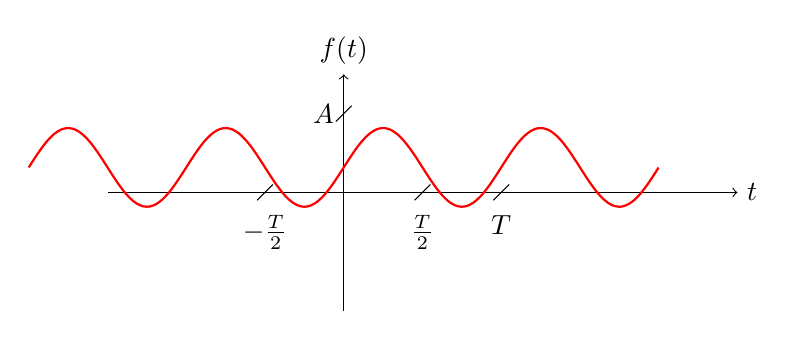
\begin{tikzpicture}
  %\draw (0,0) circle (1in);
  \draw[->] (-3.0,+0.0) -- (+5.0,+0.0) node[right] {$t$};
  \draw[->] (+0.0,-1.5) -- (+0.0,+1.5) node[above] {$f(t)$};
  %\draw[-,red, thick] (-2.5,+0.0) -- (+0.0,+0.0);
  %\draw[-] (-1.0-0.1,-0.1)--(-1.0+0.1,0.1) node[midway, below, outer sep=10pt,align=center] {$-\frac{T}{2}$};
  \draw[-] (-1.0-0.1,-0.1)--(-1.0+0.1,0.1) node[midway, below, outer sep=5pt,align=center] {$-\frac{T}{2}$};
  \draw[-] (+1.0-0.1,-0.1)--(+1.0+0.1,0.1) node[midway, below, outer sep=5pt] {$\frac{T}{2}$};
  \draw[-] (+2.0-0.1,-0.1)--(+2.0+0.1,0.1) node[midway, below, outer sep=5pt] {$T$};
  \draw[-] (-0.1,1.0-0.1)--(+0.1,1.0+0.1) node[midway, left] {$A$};
  
  \draw[scale=1.0,domain=-4:4.0,samples=100,smooth,variable=\x,red,thick] plot ({\x},{1.0/3.141592+1.0/2.0*sin(\x*180.0/3.141592*1.0*3.141592/1.0)});
  \end{tikzpicture}
\end{figure}

W przypadku sumowania do $k_{max}=2$ otrzymujemy 

\begin{figure}[H]
  \centering
  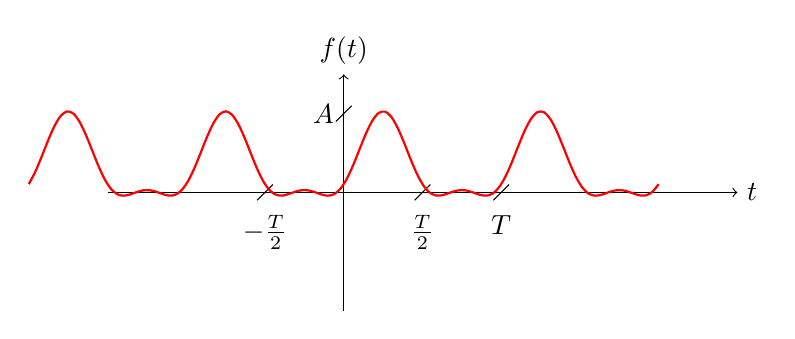
\begin{tikzpicture}
  %\draw (0,0) circle (1in);
  \draw[->] (-3.0,+0.0) -- (+5.0,+0.0) node[right] {$t$};
  \draw[->] (+0.0,-1.5) -- (+0.0,+1.5) node[above] {$f(t)$};
  %\draw[-,red, thick] (-2.5,+0.0) -- (+0.0,+0.0);
  %\draw[-] (-1.0-0.1,-0.1)--(-1.0+0.1,0.1) node[midway, below, outer sep=10pt,align=center] {$-\frac{T}{2}$};
  \draw[-] (-1.0-0.1,-0.1)--(-1.0+0.1,0.1) node[midway, below, outer sep=5pt,align=center] {$-\frac{T}{2}$};
  \draw[-] (+1.0-0.1,-0.1)--(+1.0+0.1,0.1) node[midway, below, outer sep=5pt] {$\frac{T}{2}$};
  \draw[-] (+2.0-0.1,-0.1)--(+2.0+0.1,0.1) node[midway, below, outer sep=5pt] {$T$};
  \draw[-] (-0.1,1.0-0.1)--(+0.1,1.0+0.1) node[midway, left] {$A$};
  
  \draw[scale=1.0,domain=-4:4.0,samples=100,smooth,variable=\x,red,thick] plot ({\x},{1.0/3.141592+1.0/2.0*sin(\x*180.0/3.141592*1.0*3.141592/1.0)-2.0/(3.0*3.141592)*cos(\x*180.0/3.141592*2.0*3.141592/1.0)});
  \end{tikzpicture}
\end{figure}

W przypadku sumowania do $k_{max}=4$ otrzymujemy 

\begin{figure}[H]
  \centering
  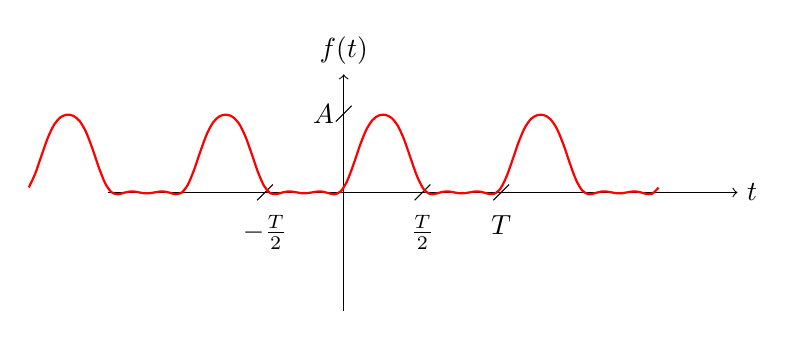
\begin{tikzpicture}
  %\draw (0,0) circle (1in);
  \draw[->] (-3.0,+0.0) -- (+5.0,+0.0) node[right] {$t$};
  \draw[->] (+0.0,-1.5) -- (+0.0,+1.5) node[above] {$f(t)$};
  %\draw[-,red, thick] (-2.5,+0.0) -- (+0.0,+0.0);
  %\draw[-] (-1.0-0.1,-0.1)--(-1.0+0.1,0.1) node[midway, below, outer sep=10pt,align=center] {$-\frac{T}{2}$};
  \draw[-] (-1.0-0.1,-0.1)--(-1.0+0.1,0.1) node[midway, below, outer sep=5pt,align=center] {$-\frac{T}{2}$};
  \draw[-] (+1.0-0.1,-0.1)--(+1.0+0.1,0.1) node[midway, below, outer sep=5pt] {$\frac{T}{2}$};
  \draw[-] (+2.0-0.1,-0.1)--(+2.0+0.1,0.1) node[midway, below, outer sep=5pt] {$T$};
  \draw[-] (-0.1,1.0-0.1)--(+0.1,1.0+0.1) node[midway, left] {$A$};
  
  \draw[scale=1.0,domain=-4:4.0,samples=100,smooth,variable=\x,red,thick] plot ({\x},{1.0/3.141592+1.0/2.0*sin(\x*180.0/3.141592*1*3.141592/1.0)-2.0/(3.0*3.141592)*cos(\x*180.0/3.141592*2.0*3.141592/1.0)-2.0/(15.0*3.141592)*cos(\x*180.0/3.141592*4.0*3.141592/1.0)});
  \end{tikzpicture}
\end{figure}

W przypadku sumowania do $k_{max}=6$ otrzymujemy 

\begin{figure}[H]
  \centering
  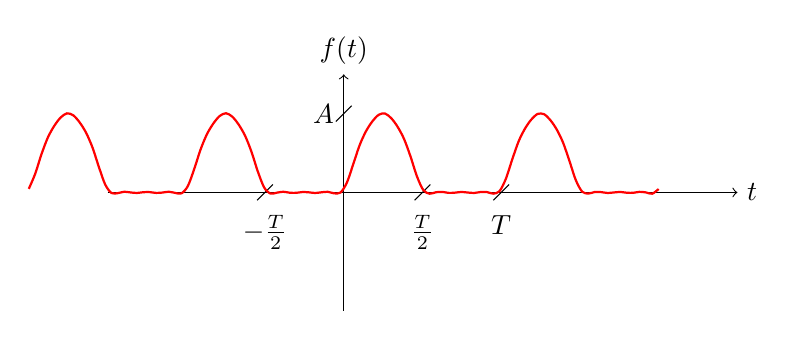
\begin{tikzpicture}
  %\draw (0,0) circle (1in);
  \draw[->] (-3.0,+0.0) -- (+5.0,+0.0) node[right] {$t$};
  \draw[->] (+0.0,-1.5) -- (+0.0,+1.5) node[above] {$f(t)$};
  %\draw[-,red, thick] (-2.5,+0.0) -- (+0.0,+0.0);
  %\draw[-] (-1.0-0.1,-0.1)--(-1.0+0.1,0.1) node[midway, below, outer sep=10pt,align=center] {$-\frac{T}{2}$};
  \draw[-] (-1.0-0.1,-0.1)--(-1.0+0.1,0.1) node[midway, below, outer sep=5pt,align=center] {$-\frac{T}{2}$};
  \draw[-] (+1.0-0.1,-0.1)--(+1.0+0.1,0.1) node[midway, below, outer sep=5pt] {$\frac{T}{2}$};
  \draw[-] (+2.0-0.1,-0.1)--(+2.0+0.1,0.1) node[midway, below, outer sep=5pt] {$T$};
  \draw[-] (-0.1,1.0-0.1)--(+0.1,1.0+0.1) node[midway, left] {$A$};
  
  \draw[scale=1.0,domain=-4:4.0,samples=100,smooth,variable=\x,red,thick] plot ({\x},{1.0/3.141592+1.0/2.0*sin(\x*180.0/3.141592*1*3.141592/1.0)-2.0/(3.0*3.141592)*cos(\x*180.0/3.141592*2.0*3.141592/1.0)-2.0/(15.0*3.141592)*cos(\x*180.0/3.141592*4.0*3.141592/1.0)-2.0/(35.0*3.141592)*cos(\x*180.0/3.141592*6.0*3.141592/1.0)});
  \end{tikzpicture}
\end{figure}

W przypadku sumowania do $k_{max}=12$ otrzymujemy 

\begin{figure}[H]
  \centering
  \begin{tikzpicture}
  %\draw (0,0) circle (1in);
  \draw[->] (-3.0,+0.0) -- (+5.0,+0.0) node[right] {$t$};
  \draw[->] (+0.0,-1.5) -- (+0.0,+1.5) node[above] {$f(t)$};
  %\draw[-,red, thick] (-2.5,+0.0) -- (+0.0,+0.0);
  %\draw[-] (-1.0-0.1,-0.1)--(-1.0+0.1,0.1) node[midway, below, outer sep=10pt,align=center] {$-\frac{T}{2}$};
  \draw[-] (-1.0-0.1,-0.1)--(-1.0+0.1,0.1) node[midway, below, outer sep=5pt,align=center] {$-\frac{T}{2}$};
  \draw[-] (+1.0-0.1,-0.1)--(+1.0+0.1,0.1) node[midway, below, outer sep=5pt] {$\frac{T}{2}$};
  \draw[-] (+2.0-0.1,-0.1)--(+2.0+0.1,0.1) node[midway, below, outer sep=5pt] {$T$};
  \draw[-] (-0.1,1.0-0.1)--(+0.1,1.0+0.1) node[midway, left] {$A$};
  
  \draw[scale=1.0,domain=-4:4.0,samples=100,smooth,variable=\x,red,thick] plot ({\x},{1.0/3.141592+1.0/2.0*sin(\x*180.0/3.141592*1*3.141592/1.0)-2.0/(3.0*3.141592)*cos(\x*180.0/3.141592*2.0*3.141592/1.0)-2.0/(15.0*3.141592)*cos(\x*180.0/3.141592*4.0*3.141592/1.0)-2.0/(35.0*3.141592)*cos(\x*180.0/3.141592*6.0*3.141592/1.0)-2.0/(63.0*3.141592)*cos(\x*180.0/3.141592*8.0*3.141592/1.0)-2.0/(99.0*3.141592)*cos(\x*180.0/3.141592*10.0*3.141592/1.0)-2.0/(143.0*3.141592)*cos(\x*180.0/3.141592*12.0*3.141592/1.0)});
  \end{tikzpicture}
\end{figure}

W granicy sumowania do $k_{max}=\infty$ otrzymujemy oryginalny sygnał.

\end{task}